\documentclass[msc,oneside]{ubcthesis}%msc, phd, masc, ma, or meng

% ================================================================================
% CHANGE THE FOLLOWING ACCORDING TO YOUR PROGRAM/THESIS
% ================================================================================
\institution{The University Of British Columbia}
\faculty{Unit 5}
\institutionaddress{Okanagan}

% For an Honours thesis, use \documentclasss[msc,oneside]{ubcthesis} above and
% uncomment and modify the next line:
\degreetitle{B.Sc. Computer Science Honours}

\title{Honours Computer Science Thesis}
\subtitle{\emph{rally}, a one stop-shop for all reddit data}
\author{Kevin J. Eger}
\copyrightyear{2016}
\submitdate{April 2016} % date of approved thesis
\program{Computer Science}%or Mathematics, or Interdisciplinary Studies

% ================================================================================


\usepackage{ubcostyle} %loads packages


% ===================================================================
% CHANGE THE FOLLOWING COMMANDS ACCORDING TO YOUR NEEDS
% ===================================================================
\newcommand{\R}{\mathbb{R}}   %real number
\newcommand{\Z}{\mathbb{Z}}   %integers
\newcommand{\C}{\mathbb{C}}   %complex numbers

\newcommand{\dom}{\operatorname{dom}}
\providecommand{\TT}[1]{\Theta\left(#1\right)} % big-Theta
\providecommand{\OO}[1]{\mathcal{O}\left(#1\right)} % big-Oh
\setlength{\parskip}{1em}
% ===================================================================

%Uncomment the next line if there are more than one appendix
%\renewcommand*\appendixname{Appendices}

\usepackage{graphicx}
\graphicspath{ {images/} }
\usepackage[section]{placeins}

\usepackage{xcolor}
\usepackage{listings}
\usepackage[T1]{fontenc}
\usepackage{xparse}
\usepackage[linesnumbered,ruled,vlined]{algorithm2e}
\usepackage{csvsimple}

\lstset{	
	language=PHP,
    breaklines=true,
    postbreak=\raisebox{0ex}[0ex][0ex]{\ensuremath{\color{red}\hookrightarrow\space}},
    tabsize=2
}

\lstdefinelanguage{PHP}{
	commentstyle = \color{gray},
    extendedchars = \true,
    inputencoding = utf8x,
    keepspaces = true,
    keywordstyle = \bfseries,
    morekeywords={function,return},
}

\NewDocumentCommand{\sqlword}{v}{%
\texttt{\textcolor{gray}{#1}}%
}

\NewDocumentCommand{\inlinemathword}{v}{%
\texttt{#1}%
}

\SetKwInOut{Input}{input}\SetKwInOut{Output}{output}

\begin{document}

% This starts numbering in Roman numerals as required for the thesis
% style.
\frontmatter                    % Mandatory

% The order of the following components should be preserved.  The order
% listed here is the order currently required by FoGS.
\maketitle                      % Mandatory

\begin{abstract}                % Mandatory -  maximum 350 words
Reddit is \emph{the front page of the internet}, a slogan the company has coined and rightfully lived up to. It is a website which brings together members of all communities in a similar style to a typical forum but with much more structure and a lot more traffic. The open nature of Reddit generates a large amount of traffic, averaging over 200 million unique visitors a month. With such traffic screams the demand for data analysis through a human-interpretable medium which this thesis covers. Data analysis on reddit has been done before however this thesis focuses on bringing the data gathered in to a easily consumable format. Techniques for consuming less apparent analysis and alternative browsing techniques are covered. We will explore the implementation and results of querying the reddit API, generating aggregate statistics, querying large data dumps of historic reddit data with \emph{Google BigQuery}, analyzing and labelling the content of Reddit using \textit{Google Cloud Vision}'s image recognition and the use of unsupervised machine learning to draw powerful conclusions.
\end{abstract}

\newpage
\phantomsection \label{tableofcontent}%set anchor at right location
\addcontentsline{toc}{chapter}{\contentsname}
\tableofcontents                % Mandatory: generate toc
\newpage 
\phantomsection \label{listoftab}%set anchor at right location
\addcontentsline{toc}{chapter}{\listtablename}
\listoftables                   % Mandatory if thesis has tables
\newpage
\phantomsection \label{listoffig}%set anchor at right location
\addcontentsline{toc}{chapter}{\listfigurename}
\listoffigures                  % Mandatory if thesis has figures


\chapter{Acknowledgements}      % Optional
Work on this thesis was widely facilitated with help from Dr. Ramon Lawrence through weekly meetings where ideas and progress were discussed extensively. It is also important to acknowledge Dr. Jeff Andrews for his support in advising on machine learning techniques which were implemented as described later.



% Any other unusual prefactory material should come here before the
% main body.

% Now regular page numbering begins.
\mainmatter\setlength{\parskip}{1em}

% Parts are the largest structural units, but are optional.
%\part{Thesis}

% Chapters are the next main unit.
\chapter{Introduction}
High level overview and motivation for developing this thesis.

\section{Reddit}
Reddit is a a news and entertainment website whose content is sustained by members of the community. Users submit text posts or direct links similar to a typical forum setting. Registered users can vote on submissions bringing order to the posts which yields an ordered online bulletin board. Furthermore, what makes Reddit unique is that content is subsectioned into different areas of interest called ``subreddits''. Some of the top subreddits include \textit{movies}, \textit{funny}, \textit{AskReddit}, \textit{food} and \textit{news}. As of March 3rd, 2016 Reddit had 231,625,384 unique users a month viewing a total of 7,517,661,034 pages. The company was founded 10 years ago and has quickly become the most central place on the internet to partake in conversation or consume a wide array of content.

\section{Motivation}
For years data analytics has been used in many industries to give companies and organizations better business decisions and verification of their models and structures. Whether they are mining huge data sets, looking at specific use cases or aiming to prove or disprove a theory, companies and organizations alike aim to do one thing: identify and discover patterns, relationships and inferences that are not immediately apparent.
\par
An early motivator for this thesis was some existing technology for Twitter insights. The community-content driven nature of Twitter parallels that of Reddit. There has already been a lot of academic research and production level software released for Twitter data management, pattern identification and tracking. The existing infrastructure in the Twitter space can be largely replicated and modified to suit Reddit, an effort which this thesis focuses on starting.

\chapter{Background}
To best understand this thesis and the work done, it is necessary to first be introduced to the relevant technologies and key terms which will be heavily referenced and built upon.

\section{Terms and Definitions}
TODO

\section{Reddit}

\subsection{History}
The company was founded by two new graduates of the \textit{University of Virginia}, Steve Huffman and Alexis Ohanian, in June 2005 \citep{Guardian}. After a couple years of growth, Reddit's traffic exploded and the service went viral. The creators were quick to release Reddit Gold, which offered new features and usability improvements providing the company with a primary source of income.

\subsection{Community}
Reddit thrives on its open nature and diverse content fully generated by the community \citep{Atlantic}. The demographics Reddit serves allows for a wide range of subject areas thus having the ability for smaller communities to digest their niche content. Subreddits provide a very unique opportunity by raising attention and fostering discussion that may not be seen as mainstream and covered by other news or entertainment mediums.
\par{}
Reddit as a company and as a community has been known for several philanthropic projects both short and long term. A few of notable efforts are as follows:
\begin{itemize}
\item{Users donated \$185,356 to Direct Relief for Haiti after the earthquake that struck the country in January 2010}
\item{Reddit donates 10\% of it's yearly annual ad revenue to non-profits voted upon by its users \citep{RedditBlog}}
\item{Members from Reddit donated over \$600,000 to DonorsChoose in support of Stephen Colbert's March to Keep Fear Alive \citep{DonorsChoose}}
\end{itemize}

\chapter{Technical Stack}
\textit{Rally} is a project that explores many different types of data access, processing techniques and display forms. Due to the nature of web applications, it is no surprise that \textit{Rally} is implemented with modular programming in mind. Several key components outlined below are what will allow this project to be easily continued and built on. The technical stack is broken in to components as follows.

\section{Laravel}
Laravel is a \textit{PHP} web application framework with expressive, elegant syntax \citep{Laravel}. Laravel is designed primarily with the motive of removing the repetitive and often painful part of building trivial common tasks to a majority of web projects (ie: authentication, routing, sessions, etc.). Laravel aims to make the development process a pleasing one for the developer without sacrificing application functionality \citep{Laravel}. The accessible and powerful framework was chosen for it's existing familiarity and power to implement a project spanning many domains.

\subsection{MVC}
Laravel follows the traditional Model-View-Controller design pattern. Models interact with the database through the \textit{Eloquent} ORM providing an object oriented handle on information. Controllers handle the requests and retrieving data by leveraging the models. Views render the web pages and are returned to the user.
\par
This intrinsic design pattern was followed tightly alongside the addition of a repository layer. As discussed later, \textit{Rally} interacts with several external resources such as the Reddit API and the \textit{Google Cloud Platform}. These external resources house gigabytes of data thus storing them locally and accessing them through a model is counterproductive. To retain the structure of the MVC framework, a repository layer is built on top of the models. This allows for the convenience of a seemingly object oriented interaction with data outside of the application. Not only does it allow for convenient method calls but also abstracts logic away from the controllers, leaving them as slim as possible. This is a vital design philosophy to web development as it modularizes code to ensure a more rigid flow and testable code-base. Basic examples from \textit{Rally} utilizing each level of the MVC framework as well as the repository layer are as follows:
\par{}
% Model Example
\begin{figure}[!htb]
\begin{center}
\begin{lstlisting}
$cluster_image = Cluster::where("name", $subreddit)->first();
\end{lstlisting}
\end{center}
\caption[Example of Model]{
A basic example of retrieving the first \textit{Cluster} model where the name field matches.}
\end{figure}

% View Example
\begin{figure}[!htb]
\begin{lstlisting}
<select name="labels" . . . multiple="">
	@foreach($labels as $label)
		<option value="{{ $label }}">{{ $label }}</option>
	@endforeach
</select>
\end{lstlisting}
\caption[Example of View]{
A basic example demonstrating how objects passed to the view are utilized and iterated over to display the options for the index page of \textit{Content Search}. \textit{Laravel} leverages an HTML templating engine called \textit{Blade} which allows for convenient variable dumping and interaction.}
\end{figure}

% Controller Example
\begin{figure}[!htb]
\begin{lstlisting}
public function show(Request $request)
{
	$subreddit = $request->get("subreddit");
	$about = $this->phpraw->aboutSubreddit($subreddit);
	
	return response()->view("subreddit.show", [
		"subreddit" => $subreddit,
		"about"     => $about->data,
		"tagline"   => "A look at /r/" . $subreddit
	]);
}
\end{lstlisting}
\caption[Example of Controller]{
A basic example of the show() functions in the subreddit controller. This method retrieves the necessary data, then sends the data to a blade view (subreddit/show.blade.php) and returns a rendered instance of that view.}
\end{figure}

% Repository Example
As mentioned above, the repository layer is utilized primarily to wrap auxiliary data sources. This gives them a similar feel and interaction as a traditional model. Seen in figure \ref{fig:repository}, a RedditorRepository instance is injected in to the RedditorsController class which is then used in its internal functions to gather data using the phpRaw Reddit API wrapper in a chainable method technique identical to a traditional model.
\begin{figure}[!htb]
\begin{lstlisting}
protected $redditor;

public function __construct(RedditorRepository $redditor)
{
	$this->redditor = $redditor;
}
...
public function show(Request $request)
{
	$user = $request->redditor;
	$subreddits = $this->redditor->getUserSubmitted($user)->getSubredditsList();
	...
}
\end{lstlisting}
\caption[Example of Repository]{
Code snippets from the Redditor Controller which leverages the power of a repository layer to make chain-able function calls to an auxiliary data source.}
\label{fig:repository}
\end{figure}

\section{Storage}
Databases used to house the necessary persistent information for the application.

\subsection{MySQL}
MySQL is an open-source relational database management system (DBMS). In Laravel, it is the default DBMS largely because of it's \textit{plug and play} nature. The MySQL database is what houses the caching layer as described in detail in the [insert section] section. A visual representation of the schema is depicted as follows:

\begin{figure}[!htb]
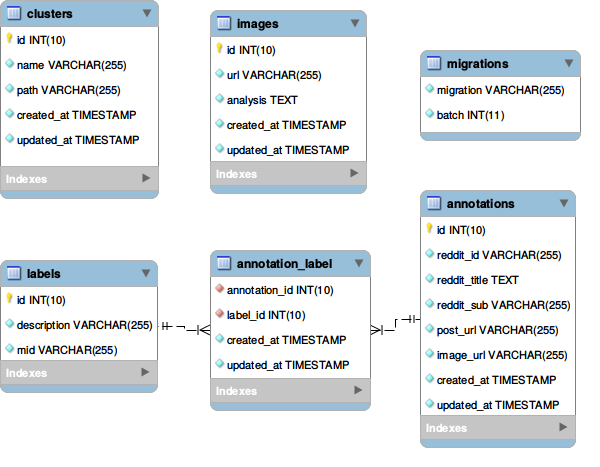
\includegraphics[width=\textwidth]{mysql_er_April_2.png}
\caption[MySQL Database schema]{
An ER diagram representing the MySQL database schema.}
\end{figure}

\subsection{BigQuery}
Querying massive datasets can not only be time consuming but expensive without the right hardware, infrastructure and software. \textit{Google} alleviates this problem with \textit{BigQuery}, an incredibly fast cloud-based storage platform. It is infrastructure as a service (IaaS) that handles all the hard work of both creating and accessing large data sets. Using the processing power of \textit{Google}, a user can get up and running with \textit{BigQuery} in a matter of minutes. The service can be used via their web UI, command-line tool or the REST API using one of the many client libraries. 
\par
Five months ago, user /u/Stuck{\_}In{\_}the{\_}Matrix of reddit collected all Reddit submission data from 2006 to 2015. He had effectively bundled 200 million submission objects, each with score data, author, title, self{\_}text, media tags and all the other attributes that are normally available via the Reddit API. The dataset complemented the Reddit comment corpus he released a couple months prior. When the data was initially made publicly available, he released it as a torrent where developers interested in using it could download their own local copies. Developers were all downloading the data for use either on their local machines or a cloud server. The problem with this is even with one of the most powerful desktop computers, loading the entire dataset into RAM was not feasible. Search times and joining (cross table) operations were expensive. 
\par
Conveniently soon after the release of this torrent, one of the lead engineers of \textit{Google BigQuery}, Felipe Hoffa, uploaded the data to \textit{BigQuery} and made the dataset publicly available. Each month, the dataset is updated with the latest information collected from the Reddit API.
\par
With the convenience of BigQuery, it is now possible to query gigabytes of history Reddit data in a matter of seconds. Listed below are a few of the integral queries used in \textit{Rally}, their sizes and the execution time.

% Best time to post on Reddit
\begin{figure}[H]
\begin{lstlisting}
SELECT subreddit, total, sub_hour, num_gte_3000
FROM (
	SELECT
		HOUR(SEC_TO_TIMESTAMP(created - 60*60*5)) as sub_hour,
		SUM(score >= 3000) as num_gte_3000,
		SUM(num_gte_3000) OVER(PARTITION BY subreddit) total, subreddit,
	FROM [fh-bigquery:reddit_posts.full_corpus_201509]
	WHERE YEAR(SEC_TO_TIMESTAMP(created))=2015
	GROUP BY sub_hour, subreddit
	ORDER BY subreddit, sub_hour
)
WHERE total>700
ORDER BY total DESC, sub_hour
\end{lstlisting}
\caption[Query finding the best hours to post on Reddit]{
The BigQuery SQL for finding the best hours to post on Reddit. This query processes 5.00GB across one table in roughly 8 seconds (~1.5 seconds when cached)}
\end{figure}

% Activity on Reddit over time
\begin{figure}[H]
\begin{lstlisting}
SELECT RIGHT('0'+STRING(peak),2)+'-'+subreddit, hour, c 
FROM (
  SELECT subreddit, hour, c, MIN(IF(rank=1,hour,null)) 
  OVER(PARTITION BY subreddit) peak 
  FROM (
    SELECT subreddit, HOUR(SEC_TO_TIMESTAMP(created_utc)) hour, COUNT(*) c, ROW_NUMBER() 
    OVER(PARTITION BY subreddit ORDER BY c ) rank 
    FROM [fh-bigquery:reddit_comments.2015_08] 
    WHERE subreddit IN (%subreddits) 
    AND score>2 
    GROUP BY 1, 2 )
    )
ORDER BY 1,2
\end{lstlisting}
\caption[Query finding the best hours to post on Reddit]{
Viewing activity (number of submissions) on subreddits over time. The wildcard \textit{\%subreddits} is replaced with a string comma-separated list of subreddits. This query processes 1.49GB across one table in roughly 2.5 seconds (~1.1 seconds when cached)}
\end{figure}

\subsubsection{Facades in Laravel with Google Services}
In web programming, quite often developers will need access to static references to classes. Facades provide a static interface to such classes that are available in the application's service container. By default Laravel ships with several facades. These static proxies to underlying classes in the service container provide the benefit of a terse, expressive syntax while maintaining more testability and flexibility than traditional static methods.
\par
The facade class itself only needs to implement a single method \textit{getFacadeAccessor}. It is that method's job to define what to resolve from the container. Behind the scenes, the base facade class (which all facades must extend) makes use of a magic-method, \textit{\_\_callStatic()}, which defers calls from the facade to the resolved object. 

% Registering the service provider
\begin{figure}[H]
\begin{lstlisting}
public function register()
{
	$this->app->bind('google', function () {
		$client = new Google_Client();
		$client->useApplicationDefaultCredentials();
		$client->addScope(Google_Service_Bigquery::BIGQUERY);
		
		return new GoogleAPI($client);
	});
}
\end{lstlisting}
\caption[Registering the Google service provider]{
Registering the Google service provider and binding the facade keyworld \textit{Google} to it.}
\end{figure}

The point of registering a facade may at times seem convoluted and unnecessary. It has always been a topic of discussion amongst the PHP world and a lot of the time boils down to personal preference and code readability. The facade approach was chosen particularly for \textit{BigQuery} part of the project for a few main reasons:
\begin{itemize}
  \item Expressive syntax without sacrificing testability of code
  \item Keep class responsibility narrow and well defined
  \item Clean constructor injection to automatically connect to \textit{Google Services} and access the \textit{BigQuery API}
  \item Explicit declaration defines what the class needs and what the class does
\end{itemize}

\section{Python}
\subsection{Scipy}
[Insert chunk about Scipy]
\subsection{Matplotlib}
[Insert chunk about Matplotlib]

\chapter{Algorithms and Methods}
The sets of operations integral to the key components of \textit{Rally}.
\section{Hierarchical Clustering}
When observing an open environment, an equally interesting and powerful metric for how the community is distributed is with clustering. One of the biggest benefits of hierarchical clustering is that you don't need to already know the number of clusters in the data set. It is with hierarchical clustering that within a subreddit, we are able to detect sub-communities. Strategies for hierarchical clustering land within two groups: agglomerative and divisive. Agglomerative is a bottom up approach where each observation starts in it's own cluster and pairs are merged as you move up the hierarchy. Divisive is a top down approach where all observations begin in a single cluster and split recursively down throughout the hierarchy. 
\par
To best understand the hierarchical clustering process, we will begin by showing the end result in what is known as a dendrogram. A clustering of users amongst the subreddit \textit{/r/movies} is shown as a dendrogram in Figure \ref{fig:moviesdend}. The dendrogram is a visualization in the form of a tree that shows the order and distances of merges throughout the hierarchical clustering. It can be understood as snapshots throughout the linkage of observations. On the x axis are labels representing numbers of samples (if in brackets) or specific samples (without brackets). On the y axis are the relative distances (using the 'ward' method described later). Beginning at the bottom of the lines (near the labels), the height of the horizontal joining lines tells us about the distance at which that labelled group merged with another label or cluster. 

\begin{figure}[H]
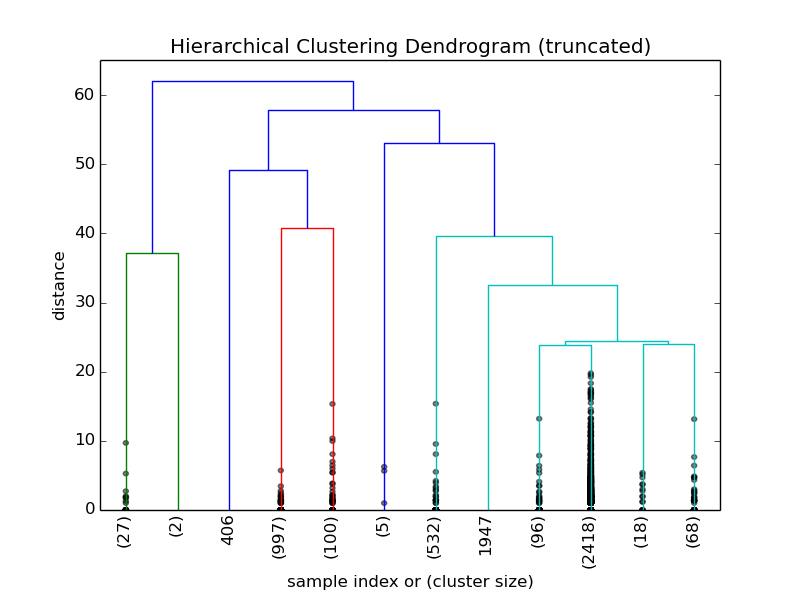
\includegraphics[width=\textwidth]{movies_dendogram.png}
\caption[Dendrogram of /r/movies]{
A dendrogram representing the hierarchical clustering amongst the subreddit \textit{/r/movies}.}
\label{fig:moviesdend}
\end{figure}

\par
For the example shown in Figure \ref{fig:moviesdend} there are 4265 samples (users) being processed. What is actually being shown is a truncated dendrogram, showing only the last 12 merges. The small black dots along the vertical lines represent joins that happened prior the the final 12. Truncation is an incredibly useful tool when plotting dendrograms. More often than not, we are only interested in the last few merges amongst the samples. The merge that carries the largest vertical distance will be the merge that attaches the most segregated groups. Again with the example in Figure \ref{fig:moviesdend} we can see three distinct groups being formed, identified by their green, red and teal colours.
\par
Before we start summarizing the process, it is sometimes easy to forget what variables map to. A list is provided here:
\begin{itemize}
\item{X: samples (n*m array), or data points or "singleton clusters"}
\item{n: number of samples}
\item{m: number of features}
\item{Z: cluster linkage array}
	\begin{itemize}
	\item{Contains the hierarchical clustering information}
	\end{itemize}
\item{k: number of clusters}
\end{itemize}
\par

\subsection{The Clustering Process}
To begin the clustering, we first gather the necessary data from \textit{Google BigQuery}. The query retrieves the most recent 300 posts for the specified subreddit. A join is then made with the \texttt{link\_id} from the inner query and a \sqlword{UNION ALL} with the comment shard tables over the past 3 months. \textit{BigQuery} does not directly support the \sqlword{UNION ALL} syntax familiar to most sql languages, but instead supports comma separated tables wrapped in a \sqlword{SELECT *}. After joining up the relations, user accounts that were deleted or made by an auto moderator are filtered out. The remaining authors are grouped by the \texttt{link\_id} and selected out by the number of times they commented on each link. The query as it is executed in the application can be seen in figure \ref{fig:clusterquery}. The query processes 9.95GB of data across a total of 4 tables and is completed between 5 and 10 seconds (depending on the subreddit under consideration).

\begin{figure}[H]
\begin{lstlisting}
SELECT author, link_id, COUNT(link_id) as cnt 
FROM ( 
  SELECT * 
  FROM 
  [fh-bigquery:reddit_comments.2016_01], 
  [fh-bigquery:reddit_comments.2015_12], 
  [fh-bigquery:reddit_comments.2015_11] 
)
WHERE link_id IN ( 
  SELECT posts.name 
  FROM [fh-bigquery:reddit_posts.full_corpus_201512] AS posts 
  WHERE posts.subreddit = (%subreddits) 
  AND posts.num_comments > 0 
  ORDER BY posts.created_utc DESC LIMIT 300 
) 
AND author != '[deleted]' 
AND author != 'AutoModerator' 
GROUP BY author, link_id 
ORDER BY author
\end{lstlisting}
\caption[BigQuery for retrieving clustering data]{
The query executed on \textit{BigQuery} to retrieve all cluster data.}
\label{fig:clusterquery}
\end{figure}

Upon retrieving the data, the X matrix needs to be generated. As a reminder, in the matrix there are n samples and m features. Our samples are authors of comments on listings and our features are each of the listings. Outlined in figure \ref{fig:responsealgo} is the algorithm for processing the raw \textit{BigQuery} response in to a usable matrix. Because the matrices can become very large in size, we are currently limiting the data gathered by using only the most recent 300 posts. Future work could focus on coming up with a preprocessing technique to predict the anticipated size of response data from \textit{BigQuery} and select an appropriate post number.

\begin{figure}[H]
	\begin{algorithm}[H]
		\SetKwComment{tcc}{// }
		\SetAlgoLined
		\Input{raw BigQuery table response}
		\Output{n * m matrix of users and submissions with comment frequency values}
   	 	\For{each row in response} 
   	 	{
   	 		\tcc{Save the frequency a user commented on a post}
   	 		values\lbrack author\rbrack\lbrack linkid\rbrack = count\;
      		\tcc{Save unique users}
			\If{user has not been seen before}{
				\tcc{Append username to users array}
				users\lbrack\rbrack = user\; 
			}
			\If{link has not been seen before}{
				\tcc{Append link to links array}
				links\lbrack\rbrack = link\; 
			}
    		}
    		\For{each user in users}
    		{
    			\For{each link in links}
    			{
    				\tcc{If a user has commented on a link}
    				\eIf{values\lbrack user\rbrack has array key link} {
    					\tcc{Set [user][link] = count}
    					result\lbrack user\rbrack\lbrack link\rbrack = values\lbrack user\rbrack\lbrack link\rbrack\;
    				}{
    					result\lbrack user\rbrack\lbrack link\rbrack = 0;
    				}
    			}
    		}
    		return result\;
    	\end{algorithm}
\caption{Preparing the \textit{BigQuery} response data for clustering}
\label{fig:responsealgo}
\end{figure}

Upon generating the X matrix, the results are dumped out to a json encoded file. The path to the json file is then passed along with a call to execute the python script.

Generating the linkage matrix Z in python with the help of \textit{scipy} is very straightforward. An \textit{(n-1)} by 4 matrix Z is returned. At the \textit{i}-th iteration, clusters with indices \textit{Z[i, 0]} and \textit{Z[i, 1]} are combined to form cluster \textit{n+i}. A cluster with an index less than n corresponds to one of the n original observations. The distance between clusters \textit{Z[i, 0]} and \textit{Z[i, 1]} is given by \textit{Z[i, 2]}. The fourth value \textit{Z[i, 3]} represents the number of original observations in the newly formed cluster. The algorithm starts with a forest of clusters. When two clusters \textit{s} and \textit{t} from this forest are combined in to a single cluster \textit{u}, \textit{s} and \textit{t} are removed from the forest and \textit{u} is added to the forest. The algorithm is complete when only one cluster remains in the forest and this cluster becomes the root. A distance matrix is maintained at each iteration. 

The \textit{d[i,j]} entry corresponds to the distance between cluster \textit{i} and \textit{j} in the original forest. At each iteration, the algorithm must update the distance matrix to reflect the distance of the newly formed cluster \textit{u} with the remaining clusters in the forest.

There are multiple methods for calculating the distance between newly formed clusters \textit{u} and \textit{v}. We elect to use the ward method. Suppose there are |u| original observations u[0],...,u[|u|-1] in cluster u and |v| original objects v[0],...,v[|v|-1] in cluster v. Recall s and t are combined to form cluster u. Let v be any remaining cluster in the forest that is not u. Given these definitions for observations and objects, the ward method calculates distance between the newly formed cluster u and v as follows in equation \ref{warddistance}. Where u is the newly joined cluster consisting of clusters s and t, v is an unused cluster in the forest, T = |v| + |s| + |t|.

\begin{equation}
\label{warddistance}
\sqrt{\frac{|v| + |s|}{T}d(v,s)^2 + \frac{|v| + |t|}{T}d(v,t)^2 - \frac{|v|}{T}d(s,t)^2}
\end{equation}

The final piece of the puzzle is vizualizing the results using a dendrogram as introduced at the beginning of this section in Figure \ref{fig:moviesdend}. As homage to the simplicity the Python package matplotlib makes this process, the full code used to vizualize the linkage matrix is outlined in Figure \ref{fig:matplotlibdend}. As we can see, by simply specifying title, label, turning parameters and p (the number of final merges to show), we produce an intuitive dendrogram with clear colour and stage distinction.

\begin{figure}[H]
\begin{lstlisting}
plt.title('Hierarchical Clustering Dendrogram (truncated)')
plt.xlabel('sample index or (cluster size)')
plt.ylabel('distance')
plt.gcf().subplots_adjust(bottom=0.15)
dendrogram(
        Z,
        truncate_mode='lastp',  # show only the last p merged clusters
        p=12,  # show only the last p merged clusters
        leaf_rotation=90.,
        leaf_font_size=12.,
        show_contracted=True,  # to get a distribution impression in truncated branches
)
# plt.show()
plt.savefig('/your/file/location/cluster.png')
\end{lstlisting}
\caption[Drawing the dendrogram using matplotlib]{
Drawing the dendrogram using matplotlib.}
\label{fig:matplotlibdend}
\end{figure}

To summarize the results of the seemingly rigorous process outlined above, a brief list follows:
\begin{itemize}
\item{horizontal lines are cluster merges}
\item{vertical lines tell you which clusters/labels were part of merge forming that new cluster}
\item{heights of the horizontal lines tell you about the distance that needed to be "bridged" to form the new cluster}
\end{itemize}
It is the distance jumps and gaps in the dendrogram that are of value when interpreting the data. When the jump is large, it indicates that two groups are being merged together that maybe shouldn't be merged. Or in other words: we have identified two potentially unique groups that form independent clusters.

\section{Image Classification}
As discussed in the implementation chapter, image recognition was employed to effectively automate and scale the labelling of media content submitted to Reddit.
\par
Human brains make vision seem very trivial, it doesn't take much effort for humans to distinguish between a jar of alphagetti and a wasps nest (a seemingly very random example but proved to actually be a difficult task). But these are very hard problems to solve with a computer, they only seem easy because our brains are incredibly good and understanding visual queues. 
\par
In the last few years the field of machine learning has made tremendous progress on addressing these difficult problems. In particular, deep convolutional neural networks can achieve reasonable performance on hard visual recognition tasks. Often matching or exceeding human performance in some domains \citep{TensorFlow}.
\par
To classify images with labels, a first attempt was made using Google TensorFlow, the recently open sourced machine learning toolkit by Google. In particular, we focused on implementing and leveraging the power of Inception-V3 \citep{DBLP:journals/corr/SzegedyVISW15} - the newest model for identifying higher level features into classes.
\par
TensorFlow is a very complex API for programmers to use either CPU, GPU or in some cases both (using CUDA) devices. The barrier to entry is quite high but upon learning the flow of data and architecture of the infrastructure is a very powerful tool. We will not go in to detail on the implementation as it is not relevant to the underlying use.
\par
Upon implementing the image recognition class using TensorFlow, an API was built that allowed for convenient and modular calls to classify images sent along as POST data. This system was optimal as it allowed for independent testing and debugging. The major downfall was the lack of speed with the implementation for analysing the image. To reduce the computation time, CUDA was used and the algorithm was altered to run in parallel on a GPU. The main struggle with this implementation was working with the TensorFlow API on a GPU that did not support the latest version of CUDA, which was the only version TensorFlow is currently (as of April 2016) targeting. 
\par
When the GPU version of the image classification was finalized and tested, computation time was cut in half but it still took anywhere between 2 and 6 seconds to analyse a single image. The results of the classification were also dissatisfying as it only achieved an accuracy of roughly 60\%. It was difficult not to give in to the sunk cost of sticking with an approach that was built over the course of a month however as discussed in the implementation section, it was undoubtedly the correct choice to abandon TensorFlow.

\chapter{Implementation}
Turning the technology into a plan and executing.
\section{phpRaw}
The Reddit API has several endpoints. It is through these endpoints where a client can retrieve posts specific to a subreddit, post a comment, moderate their account and all other actions that are normally available through the consumable web interface. For a single use or specific focus, calling the endpoints explicitly with cURL (or another client-side URL transfer) works fine but this strategy quickly fails as needs grow. Due to the wide array of endpoint calls utilized, it was necessary to develop an API wrapper that allows convenient calls to the API. Such a wrapper already existed for Python, Java, C and a few other languages but not PHP.
\par
An open source wrapper was discovered on GitHub but was no longer maintained, was not written to comply with the latest API security requirements (OAuth2) and was missing nearly half of the endpoints. Building on the work done on this API wrapper, a successful implementation was built and is what \textit{Rally} utilizes and depends on for direct Reddit data access. The GitHub repository from the point at which it was forked and built on is linked in the appendix.
\par 
Listed below are a functions from \textit{phpRaw} to give a feel for the wrapper.
% Get the user submitted data
\begin{center}
Get the user submitted data.
\end{center}
\begin{lstlisting}
$phpRaw->getUserSubmitted($user, $limit = 25, $after = null);
\end{lstlisting}

% Get the top 10 hottest listings for a specified subreddit
\begin{center}
Get the top 10 hottest listings for a specified subreddit.
\end{center}
\begin{lstlisting}
$phpRaw->getHot('funny', 10);
\end{lstlisting}
\par
\textit{phpRaw} was then modified to serve as a standalone vendor service brought in through Laravel's default dependency manager \textit{Composer}. By extracting the wrapper to a separate module, updating and maintaining the endpoints is simple as they are changed over time. Using the power of composer and package dependencies, by including the declaration as outlined in Figure \ref{fig:composer}, whenever composer is updated it automatically updates to the latest version of \textit{phpRaw}.

% Composer.json for phpRaw
\begin{figure}[H]
\begin{lstlisting}
...
"repositories": [
	{
		"name": "kevin/phpRAW",
		"type": "vcs",
		"url": "https://github.com/kevineger/phpRAW"
	}
],
...
\end{lstlisting}
\caption[Requiring phpRaw as a dependency in composer.]{
Requiring \textit{phpRaw} as a dependency for \textit{rally} in composer.}
\label{fig:composer}
\end{figure}

\section{Rally}
Rally combines user statistics, big data, subreddit analysis and RallySearch into one convenient location.
\subsection{User Statistics}
On Reddit, users have the ability to view their recent activity (comments, submissions and saved content) and link/comment karma scores. Reddit serves this information in a similar fashion to how they display submissions on their site. This technique is effective for listing out history of comments and submissions but it proves ineffective for quickly interpreting account details. To alleviate this lack of accessibility, upon entering a user name

\section{RallySearch}
RallySearch is an alternative way of consuming Reddit. Users of Reddit are very limited by the existing search functionality. Though there exists a search bar, it is incredibly ineffective and displays close to no results as intended. Reddit developers have expressed interest in improving the functionality but have not disclosed any immediate plans to do so. This portion of the thesis aims to offer an alternative to browsing Reddit by it's content in a visually pleasing and simple fashion. The name of this standalone service has been dubbed \textit{RallySearch} and as discussed later has been launched and received by the Reddit community.

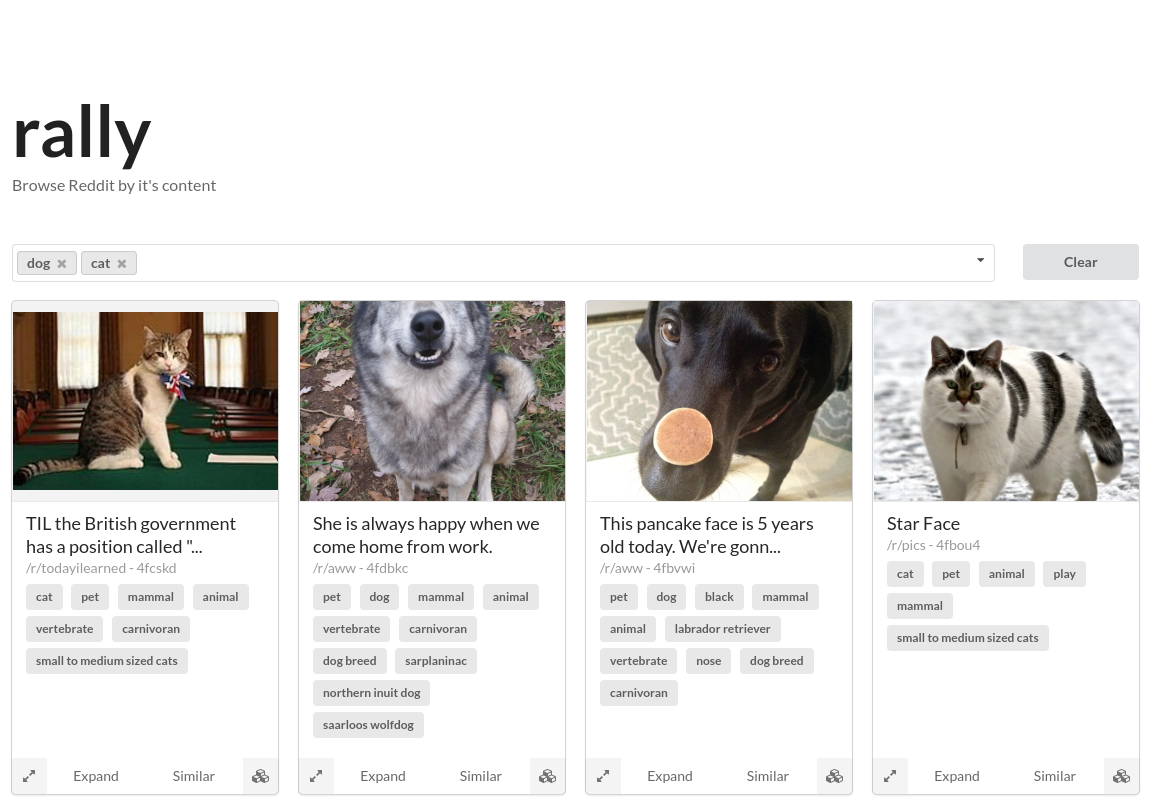
\includegraphics[width=\textwidth]{rallysearch_screenshot.png}

\subsection{Overview}
The overall point of RallySearch is to provide users with the opportunity to search Reddit by it's content - the physically linked images, videos, gifs and articles. Reddit's existing flow for browsing content does not give users the ability to search site-wide for all posts consisting of a specific object. For example, if a user wanted to view all posts pertaining to dogs and cats, they would have to manually search through all the subreddits. This may or may not contain the desired content and the only option they would have left is to perform a Google search which is even more inefficient and guarantees no degree of accuracy. Using RallySearch, labels can easily be specified using the search bar at the top and the page instantly loads all existing classified posts.

When a user first lands on the site, they are confronted with a page already populated with cards which represent posts. A card consists of the post preview image, title, labels for the image (from image recognition) as well as a few other details and options for navigation discussed later in the UI section.

In summary, top media posts on Reddit are sent through Google's Cloud Vision (Image recognition API) and results are cached. Upon giving each image (or preview in the case of videos and gifs) labels, users can easily view similar content by selecting the desired tag(s). 

\subsection{Technical Overview}
RallySearch is a slim and highly maintainable web project. It uses two external services, phpRaw (Reddit API wrapper created for this project discussed previously) and Google Cloud Vision. The technical workings of RallySearch can be divided in to two main domains: building the service and consuming the service.
\subsubsection{Building the Service}
The Google Cloud Vision API enables developers to understand the content of an image by powerful machine learning models in an easy to use REST API. Images are quickly classified into thousands of categories. Individual objects and faces can be detected within an image. The broad set of objects in images are categorized and help improve the Vision API over time as new concepts are introduced and accuracy is improved. They key feature of the API that RallySearch uses is label detection. With it, broad sets of categories are detected within in image ranging from dog breeds to wedding dresses.
\par
RallySearch is written with full modularity in mind. This is important because APIs are always subject to change over time and it incorporates two (phpRaw and Cloud Vision). The accomplish this, a Laravel Job is written which runs on a schedule. The job is executed hourly and at a high level, does the following:
\begin{itemize}
\item{Creates a new collection}
	\begin{itemize}
	\item{Laravel iterable object that wraps PHP array}
	\end{itemize}
\item{Retrieves the \textit{hottest} 100 posts on Reddit}
\item{Retrieves the \textit{top} 100 posts on Reddit}
	\begin{itemize}
	\item{Daily}
	\item{Weekly}
	\item{Monthly}
	\item{Yearly}
	\item{All time}	
	\end{itemize}
\item{Creates Annotation objects for each of the new listings}
	\begin{itemize}
	\item{Checks against database if record already exists}
	\item{Stores unique Reddit id, post url, image url (preview), post title, subreddit post was submitted to}
	\end{itemize}
\item{Labels each of the Annotations}
	\begin{itemize}
	\item{Sets labelling parameters (feature type: label and max results: 10}
	\item{Builds batch annotation image request object}
	\item{Downloads the image to be analyzed and encodes in base 64 to be sent with the request(s)}
	\item{Sends request and saves response}
	\item{Saves labels for each image, creating new Label objects when needed and reusing existing ones when applicable (An Annotation has many Labels and a Label belongs to many Annotations}
	\end{itemize}
\end{itemize}

The code for this process is slightly too long to include in the thesis but is easily accessible in the repository listed in the bibliography.

\subsubsection{Consuming the Service}
The main motivation for creating RallySearch was to offer a convenient and easy to use way of browsing Reddit. Keying in on this motivation, it was crucial users were faced with an interface that was easy to adopt and was non intrusive. More on the details of the interface can be found in the UI section, here we will go over a typical users use-case of the site.
\par
The service itself really only exists on one page, the content page. Users can browse all labelled posts by scrolling through cards and advancing through pages. For a more refined experience, a user can enter a single or multiple tags in the search bar at the top. The bar allows users to only select from a predefined list (labels which exist in the database). Upon clicking or selecting a label(s), the site loads up the appropriate content.
\par
Users are free to navigate their desired content, expand the preview for a larger view of the media and select similar tags by manually selecting those on a post or by using the "Similar" button.

\subsection{Public Reception}
Because RallySearch is a service for the community and arguably \textit{built by the community} (all the content is theirs), there was a strong desire to push the service live and generate feedback.
\par
RallySearch was made publicly available and posted to a few subreddits intended for developers and enthusiasts to give feedback and test the service. Subreddits the site was posted to include: /r/Frontend - a subreddit for front end web developers who want to move the web forward or want to learn how, /r/UsefulWebsites - a compilation of useful websites and /r/design\_critiques - a subreddit to receive critiques on a design. Over the course of just one day, submissions on /r/Frontend and /r/UsefulWebsites made it to the top submission of both subreddits and are amongst some of the top posts there over the last year. Though these subreddits are not heavily trafficked, it was a noteworthy accomplishment due the the highly opinionated, dogmatic and domineering nature of the respectful subreddits.
\par
Rather than listing all of the comments, below is a list of a few of the top comments (most upvoted) and most helpful comments that were reflected with changes and improvements.
\begin{itemize}
\item{``To be honest the accuracy of the tags blows my mind'' - /u/r\_park}
\item{``If I'm scrolled down the page, selecting the "similar" button appears to do nothing if it doesn't happen to populate more content. It also seems unintuitive that it adds more tags to my existing tags. This interaction is overall a good idea but a little unclear in terms of what it actually does.'' - /u/wayspurrchen}
\item{``The content hierarchy for the videos doesn't make a lot of sense/isn't very useful: http://i.imgur.com/RWdyvDL.png As a casual user, I'm unlikely to ever care about the permalink, and I'm most likely to care about the title. The title should also be clickable to take me to reddit. I swapped things around a bit: http://i.imgur.com/1y451Q7.png You could even put something else there like the score for that subreddit, number of comments, etc.'' - /u/wayspurrchen}
\item{``Overall this is a really killer app. I can't wait to see you polish it! :)'' - /u/wayspurrchen}
\item{``You are my new hero.'' - /u/ChaosElephant}
\item{``This is great - looks nice as well. Awesome job!
My only critique at the moment would be to have the full title reveal in some sort of tooltip or something, even just as a title attribute tooltip. At first I didn't notice the expand, or you may just think it expands the photo. It would be nice to see the full title without clicking.'' - /u/hidanielle}
\end{itemize}

It was great to get the service out there for a non-subjective set of eyes to critique, advise and shape it. Beyond having other Reddit users test the site, friends and family were also good help in offering advice and feedback from a new user (unfamiliar with Reddit) perspective. Though proper and documented user testing was not conducted, key takeaways with this group include:
\begin{itemize}
\item{Hooking up links that were expected to direct somewhere but did not initially.}
\item{Reorganizing the card structure}
\item{Altering the navigation menu for a more responsive feel}
\end{itemize}

\subsection{Analytics}
Google Analytics were implemented and utilized upon launch. This allowed for the understanding of consumer behaviour, gathering insights, tracking usage numbers and analysing performance of the site. Data tidbits from the analytics are outlined here:
\begin{itemize}
\item{736 unique visitors in the first 24 hours}
\item{0:56 seconds average session duration}
\end{itemize}
\begin{table}[H]
\begin{center}
\csvautotabular{data/osandbrowser.csv}
\caption{Operating system and browser of users}\label{tab:osandbrowser}
\end{center}
\end{table}

\begin{table}[H]
\begin{center}
\csvautotabular{data/country.csv}
\caption{Countries of users accessing the site}\label{tab:country}
\end{center}
\end{table}

\subsection{Open Source}
RallySearch is fully open source. The source code is available publicly on GitHub. There has already been a bit of interest with members of the community and the repository has had three stars from developers. The software is MIT licensed. 

\subsection{Moving Forward}
[TODO: This section]

\newpage %newpage needed otherwise pagestyle applied to previous chapter. Does not actually create a new page
\pagestyle{fancy}\chead{Bibliography}\rhead{}\cfoot{}\rfoot{\thepage}
\bibliographystyle{ubco}
\bibliography{thesis_references}%name of your .bib file

\end{document}
\endinput
